\documentclass[10pt,a4paper]{article}
\usepackage[utf8]{inputenc}
%\usepackage[engl]{babel}
\usepackage[T1]{fontenc}
\usepackage{amsmath}
\usepackage{amsfonts}
\usepackage{amssymb}
\usepackage{graphicx}
\usepackage{bm}
\usepackage[rmargin=1.5cm, lmargin=1.5cm, bmargin=2cm, tmargin=2cm]{geometry}
\usepackage{enumitem}
\setitemize{noitemsep,topsep=0pt,parsep=0pt,partopsep=0pt}


\author{Lars Schiller}
\title{Algorithm for predicting the pose of a gecko-inspired soft robot for a given reference input}


\usepackage{multicol}

\newcommand{\mbeq}{\overset{!}{=}}


\makeatletter
\renewcommand*\env@matrix[1][*\c@MaxMatrixCols c]{%
  \hskip -\arraycolsep
  \let\@ifnextchar\new@ifnextchar
  \array{#1}}
\makeatother


\begin{document}


\maketitle



Due to the fact that the behaviour of soft materials is difficult to predict with conventional methods, an algorithm based on a geometric optimization problem is presented.
The algorithm can be used to predict the actual pose of the robot for a given reference input.
Figure~\ref{fig:example} is taken as an example. The initial position is shown in black. 
The individual limbs of the robot have a certain bending angle and all feet are fixed.
Now the torso of the robot should be actuated. 
If only the bending angle of the torso is changed, the grey dashed pose is obtained. 
Obviously, the two rear feet are no longer in the same position. 
Since these feet are fixed, the robot will behave differently in reality. 
In fact, it's much more likely to take up the grey pose. 
Although the bending angles of all limbs have changed, the condition that all feet remain motionless has been fulfilled.

\begin{figure}[h]
\centering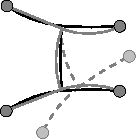
\includegraphics[scale=1]{../Pics/intro/intro.pdf}
\caption{Example Usage}
\label{fig:example}
\end{figure}



\section{Predicting the pose for a given reference input}
In order to let the robot take a pose
%, i.\,e., a position and orientation, 
the user has nine degrees of freedom at his disposal: 
the correspondending pressures for the five bending angles $\alpha_i$ of the limbs $i=1,\dots,5$ and the state of the fixation actuators $f_j \in \{0,1\}$ of the feet $j=1,\dots,4$.
For the unloaded state, a calibration function can be formulated for each limb, which maps the input pressure on the bending angle (under load, this function no longer needs to be valid).
But the input pressure can be seen as an reference for the bending angle.
Accordingly, a reference input $\bm{r}$ can be described by

\begin{equation}
\bm{\alpha}_{\textnormal{ref}} = \left[~ \alpha_{\textnormal{ref},1}~\alpha_{\textnormal{ref},2}~\alpha_{\textnormal{ref},3}~\alpha_{\textnormal{ref},4}~\alpha_{\textnormal{ref},5}~\right]^\top
\end{equation}

\begin{equation}
\bm{f} = \left[~f_1~f_2~f_3~f_4~\right]^\top
\end{equation}


\begin{equation}
\bm{r} = \left[~\bm{\alpha_{\textnormal{ref}}}^\top~\bm{f}^\top~\right].
\end{equation}

%
%\begin{equation}
%\alpha_{\textnormal{clb},i} = \textnormal{map}_i(p_i)
%\end{equation}

However, this information is not sufficient to describe the robot's actual pose.
%The exact position and orientation of at least one foot must be known.
Experiments have shown that the bending angle of a limb can vary significantly  at the same pressure level due to the softness of the used material. 
The length of a limb can also differ.
In order to describe the pose of the robot, the actual bending angles $\bm{\alpha}$: 
\begin{equation}
\bm{\alpha} = \left[ \alpha_1~\alpha_2~\alpha_3~\alpha_4~\alpha_5 \right]^\top,
\end{equation}
the actual lengths of the individual limbs $\bm{\ell$}: 
\begin{equation}
\bm{\ell} = \left[ \ell_1~\ell_2~\ell_3~\ell_4~\ell_5 \right]^\top,
\end{equation}
and the orientation of the robot's center point $\varepsilon$ must be known (see Fig.~\ref{fig:model}).
These quantities are defined as the variable to be optimized:
\begin{equation}
\bm{x} = \left[~\bm{\alpha}^\top~\bm{\ell}^\top~\varepsilon~\right]^\top.
\end{equation}

Furthermore, the position of (at least) one fixed foot ($f_j \mbeq 1$) must be known.
Then, the pose of the robot $\bm{\rho}$ can be determined under the assumption of a constant curvature by drawing arcs with the corresponding lengths and angles.
A pose can therefore be described in generally as a function of $\bm{x}$ and the position 
$\bm{P}=[\bm{p}_1~\bm{p}_2~\bm{p}_3~\bm{p}_4]^\top = [\bm{p}_x~\bm{p}_y]^\top \in \mathbb{R}^{4 \times 2}$ and state $\bm{f}$ of all feet:
\begin{equation}
\bm{\rho} = \left[\bm{x}~\bm{P}~\bm{f} \right].
\end{equation}



For a given feasible initial pose, the next pose must be determined so that all fixed feet do not move.
This can be achieved within a certain margin by deviating the bending angle from the reference angle and deviating the actual length from the nominal length.
To describe this mathematically, a new index $k$ is introduced, which assigns the quantities to a specific time step.
The new positions of the fixed feet $\bm{P}_{k}$ are assumed to be the positions from the previous pose $\bm{P}_{k-1}$.
This can be used to define the constraint for the next pose.
All newly fixed feet must have the same position as in the previous step:
\begin{equation}
\big|\big|\textnormal{diag}(\bm{f}_k)(\bm{P}_{k} - \bm{P}_{k-1})\big|\big|_2 \mbeq 0,
\label{eq:constraint}
\end{equation}


%\begin{equation}
%\bm{p}_k \left(\bm{x},~\bm{p}_{k-1},~\bm{f}_k \right).
%\end{equation}

%Please note that if this condition is met, at least one foot per time step always remains motionless.
%Thus, at least one foot position of the new pose is determined from the beginning and thus dependent on the previous pose.
%As a result, all poses of a gait are dependent on the initial position.
%\begin{equation}
%\bm{\rho}_t = \textnormal{fun}\left(\bm{x}_t,~\bm{r}_{j,0} \right).
%\end{equation}

It has already been mentioned that the bending angles $\bm{\alpha}$ and the lengths of the limbs $\bm{\ell}$ are quite variable. 
By defining 
\begin{equation}
\bm{\ell}_n = \left[ \ell_{n,1}~\ell_{n,2}~\ell_{n,3}~\ell_{n,4}~\ell_{n,5} \right]^\top
\end{equation}
as the vector containing the nominal length of each limb, it is possible to quantify the length deviation.
The orientation angles of the fixation actuators $\bm{\varphi}$ also have a certain margin.
The value of the orientation angles can be calculated as a function of $\bm{\alpha}$ and $\varepsilon$ (well, basically as a function of $\bm{x}$):
\begin{equation}
\bm{\varphi}(\bm{\alpha}, \varepsilon) = \eqref{eq:phi_calc},
\end{equation}
where the exact formula is given in the appendix~\eqref{eq:phi_calc}.
Now a objective function $\sigma$ can be formulated which quantifies the deviations of length, angle and orientation:
%\begin{equation}
%obj(\bm{x}) = w_{len}\sqrt{\sum_i \left( \ell_{n,i} - \ell_i \right)^2} 
%+ w_{ang} \sqrt{\sum_i \left( \varphi_i - \alpha_i \right)^2}
%+ w_{ori} \sqrt{\sum_i \textnormal{if}~f_i:~\left( c_{i,j-1} - c_{i, j} \right)^2}
%\label{eq:objective_function}
%\end{equation}

\begin{equation}
\sigma(\bm{x}_{k}) = %, \bm{\varphi}_{k-1}) = 
  w_\ell\big| \bm{\ell}_{k} - \bm{\ell}_n \big|_2
+ w_\alpha\big| \bm{\alpha}_{k} - \bm{\alpha}_{\textnormal{ref},k} \big|_2
+ w_\varphi \big| \textnormal{diag}(\bm{f}_k) ( \bm{\varphi}_{k} - \bm{\varphi}_{k-1}) \big|_2 .
\label{eq:objective_function}
\end{equation}
The weighting factors can be interpreted physically.
To do so, the weighting factor $w_\ell$ describes the elasticity of the limbs and $w_\alpha$ the bending stiffness of the limbs.
The term weighted by $w_\varphi$ describes the difference between the orientation of the newly fixed feet compared to the orientation in the previous time step.
This can be seen as a dimension for the torsional stiffness of the fixation actuators.
The objective function can be seen as a measure of the robot's inner stress.
Therefore it is called $\sigma$ referring to the nomenclature in mechanical engineering.
The new pose can now be determined by solving the non-linear optimization problem:

\begin{equation}
\begin{split}
&\min_{\bm{x}_k \in \mathcal{X}} ~ \sigma(\bm{x}_k) \\
&subjected~to~~~
\big|\big|\textnormal{diag}(\bm{f}_k)(\bm{P}_{k} - \bm{P}_{k-1})\big|\big|_2 = 0.
\end{split}
\end{equation}
Here  $\mathcal{X}$ describes the set of allowed values.
Each quantity inside $\bm{x}$ has bounds, which are given in the following table:

\begin{center}
\begin{tabular}{c|c|c|c}
var & $\bm{\alpha}$ & $\bm{\ell}$ & $\varepsilon$ \\ 
\hline
bounds & $\left[ \bm{\alpha_{\textnormal{ref}}}-b_\alpha,~\bm{\alpha_{\textnormal{ref}}}+b_\alpha \right]$ &
$\left[ (1-b_\ell)\bm{\ell}_n,~(1+b_\ell)\bm{\ell}_n \right]$ &
$\left[ 0^\circ,~ 360^\circ \right]$
\end{tabular}
\end{center}
These bounds can be tuned with the scalars $b_\alpha$ and $b_\ell$.
For solving the problem, for example the \texttt{SLSQP}-Algorithm provided by the python package \texttt{scipy.optimize} can be used.
Note that the evaluation of the objective function~\eqref{eq:objective_function} is quite cheap. 
The expensive part is the evaluation of the constraint function~\eqref{eq:constraint}, since the calculation of all feet positions for a given $\bm{x}$ is opulent and outlined in the appendix~\eqref{eq:F1_start}--\eqref{eq:F1_end}.

In summary, it is possible to set up a function that can predict the next pose of the robot, depending on the reference input and the previous pose:
\begin{equation}
\bm{\rho}_k = [\bm{x}_k~\bm{P}_k~\bm{f}_k] = \textnormal{fun}_{\mathcal{P}}\left( \bm{r}_k, \bm{\rho}_{k-1} \right)
\end{equation}
This function can be tuned by the parameter set $\mathcal{P}$ given in the following table:
\begin{center}
\begin{tabular}{l|l}
$\mathcal{P}$ & description \\
\hline
$b_\alpha$ & allowed absolute deviation of the bending angle to the reference angle \\
$b_\ell$ & allowed percentage deviation of the length to the nominal length \\
$w_\ell$ & costs of the length deviation / Youngs-Modulus of the material \\
$w_\alpha$ & costs of the bending angle deviation / bending stiffness of the limbs\\
$w_\varphi$ & costs of the orientation angle deviation / torsional stiffness of the fixation actuators\\
\end{tabular}
\end{center}



\begin{figure}
\centering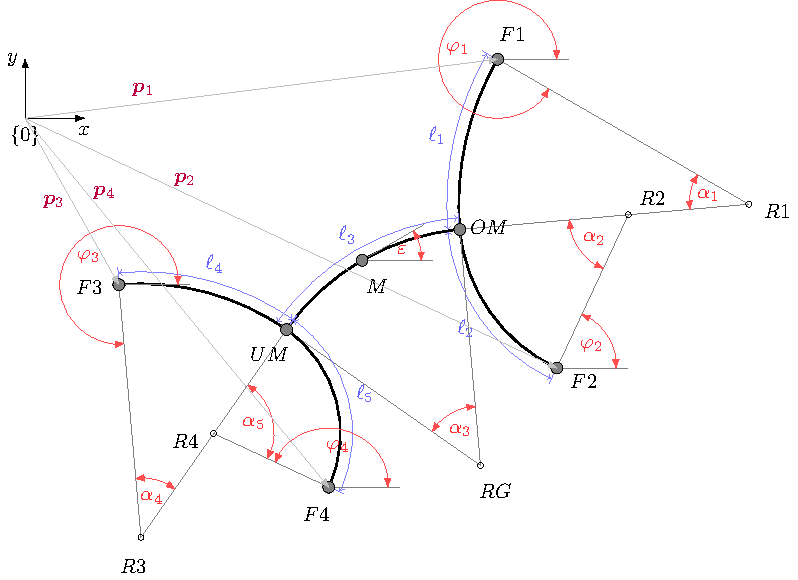
\includegraphics[scale=1]{../Pics/model/model.pdf}
\caption{Nomencalture}
\label{fig:model}
\end{figure}


\section{Finding optimal gait patterns}

%Der vorgesttele Algorithmus kann nun dazu verwendet werden neue Laufmuster zu finden.
%Da er die Möglichkeit bietet vorherzusagen, welche Pose der Roboter bei gegebenem Referenz Input einnehmen wird, ist er durch rekursive Anwendung in der Lage alle zugehörigen Posen des Roboters zu einer Sequenz von Referenz Inputs zu prädiktieren.
%

The presented algorithm can now be used to find new gait patterns.
Since it provides the ability to predict the robot's pose for a given reference input, it is also able to predict all associated poses to a sequence of reference inputs by recursive application.

%Allerdings wird eine gültige Initialpose benötigt, um den vorgestellten Algorithmus rekursiv anwenden zu können.
%Gültig in dem Sinne, dass die Längen und Biegewinkel der Glieder innerhalb des gültigen Bereichs liegen.
%Die Bedingung~\eqref{eq:constraint}, dass die im vorhergegangenen Schritt fixierten Füße nicht bewegt werden dürfen, ist an dieser Stelle hinfällig, da kein vorhergegangener Schritt existiert.
%Zur Berechnung einer gültigen Initialpose können initiale Biegewinkel $\bm{\alpha}_0$, initiale Gliederlängen $\bm{\ell}_0$ und Orientierung $\varepsilon_0$ frei gewählt werden.
%Dabei empfiehlt es sich für die Gliederlängen $\bm{\ell}_0 = \bm{\ell}_n$ zu wählen, da so die "innere Spannung" der Initialpose $\sigma(\bm{x}_0) = 0$ ist.
%Die Fußpositionen $\bm{P}_0$ ergeben sich dann durch Anwendung der Gleichungen~\eqref{eq:F1_start}--\eqref{eq:F1_end}.
%Dabei muss die initiale Koordinate des vorderen linken Fußes $\bm{p}_{1,0}$ vorgegeben werden.

However, a valid initial pose is required to apply the presented algorithm recursively.
Valid in the sense that the lengths and bending angles of the limbs are within the valid range.
The condition~\eqref{eq:constraint}, that the feet fixed in the previous step may not be moved, is void at this point, since no previous step exists.
To calculate a valid initial pose, initial bending angles $\bm{\alpha}_0$, initial limb lengths $\bm{ell}_0$ and orientation $\varepsilon_0$ can be freely defined.
For the limb lengths $\bm{\ell}_0 = \bm{\ell}_n$ is recommended, as the " inner stress " of the initial pose is $\sigma(\bm{x}_0) = 0$.
The feet positions $\bm{P}_0$ result then by application of equations~\eqref{eq:F1_start}--\eqref{eq:F1_end}.
Thereby the initial coordinate of the front left foot $\bm{p}_{1,0}$ must be provided.


\begin{equation}
\bm{\rho}_0 = 
\left[
\begin{array}{c|c|c}
\bm{x}_0 & \bm{P}_0 & \bm{f}_0
\end{array}
\right]
=
\left[
\begin{array}{c|c|c}
\bm{\alpha}_0 ~ \bm{\ell}_n ~ \varepsilon_0  & 
\bm{P}(\bm{\alpha}_0, \bm{\ell}_n, \varepsilon_0, \bm{p}_{1,0}) & 
1~0~0~0
\end{array}
\right]
\end{equation}

%Ein Laufmuster besteht aus einer ebensolchen Sequenz aus Posen, die in Dauerschleife eingenommen werden.
%Um nun eine optimale Abfolge von Referenz Inputs zu finden, muss erst einmal definiert werden, was optimal ist.
%Dies kommt ganz darauf an, welche Art von Laufmuster gesucht wird. 
%im Folgenden werden zwei Beispiele vorgestellt.


A gait pattern consists of a sequence of poses taken in a loop with a certain number of cycles.
To find an optimal sequence of reference inputs, it is first necessary to define what is optimal.
This depends entirely on the type of gait pattern we are looking for. 
Two examples are presented below.


\subsection{Straight Gait}
%Es ist sinnvoll anzunehmen, dass ein symmetrisches Laufmuster am ehesten zu einem geradlinigen Gang führen wird.
%Symmetrisch in dem Sinne, dass auf eine bestimmte Pose stets die zur Längsache gespiegelte Pose folgt.
%Außerdem sind die Fixierungszustände der Füße ebenfalls von vornherein bekannt, da für einen symmetrischen Gang stets die diagonal gegenüberliegenden Füße fixiert sein müssen (siehe vorhergegangene Forschungsarbeiten - \cite{PA_Schiller}).
%Damit besitzt das Laufmuster nur fünf Unbekannte, nämlich die Referenzwinkel der ersten Pose -- alle weiteren Posen innerhalb des Laufmusters sind Spiegelbilder.

It is reasonable to assume that a symmetrical gait pattern will most likely lead to a straigth gait.
Symmetrical in the sense that a certain pose is always followed by a pose mirrored to the longitudinal axis.
In addition, the state of fixation of the feet is also known from the outset, since the diagonally opposite feet must always be fixed for a symmetrical gait (see previous research work - \cite{PA_Schiller}).
Thus, the running pattern has only five unknowns, namely the reference angles of the first pose -- all other poses within the gait pattern are mirror images.
Therefore the variable to be optimized can be defined as:
\begin{equation}
\bm{y} = 
\begin{bmatrix}
\alpha_{\textnormal{ref},1}& \alpha_{\textnormal{ref},2}&\alpha_{\textnormal{ref},3}&\alpha_{\textnormal{ref},4}&\alpha_{\textnormal{ref},5}
\end{bmatrix} .
\end{equation}

%Mit diesen Annahmen kann eine Struktur für das noch unbekannte Laufmuster für den geradlinigen Gang mit $n$ Zyklen $\bm{R}_\mathcal{S}^n \in \mathbb{R}^{2n \times 9} $ vorgegeben werden:

With these assumptions a structure for the still unknown straight gait pattern with $n$ cycles $\bm{R}_\mathcal{S}^n \in \mathbb{R}^{2n \times 9} $ can be given as:
\begin{equation}
\bm{R}_\mathcal{S}^n(\bm{y})
=
\left[
\begin{array}{c}
\bm{r}_1 \\
\bm{r}_2 \\
\hline
\bm{r}_3 \\
\bm{r}_4 \\
\hline
\vdots \\
\hline
\bm{r}_{2n-1} \\
\bm{r}_{2n} \\
\end{array}
\right]
=
\left[
\begin{array}{ccccc cccc}
y_1&y_2& y_3&y_4&y_5&1&0&0&1 \\
y_2&y_1&-y_3&y_5&y_4&0&1&1&0 \\ 
\hline
y_1&y_2& y_3&y_4&y_5&1&0&0&1 \\
y_2&y_1&-y_3&y_5&y_4&0&1&1&0 \\
\hline
\vdots&\vdots&\vdots&\vdots&\vdots&\vdots&\vdots&\vdots&\vdots \\
\hline
y_1&y_2& y_3&y_4&y_5&1&0&0&1 \\
y_2&y_1&-y_3&y_5&y_4&0&1&1&0 \\
\end{array}
\right] .
\label{eq:gait_ptrn}
\end{equation}



%Soll der Roboter geradeaus Laufen, so ist es optimal die Distanz von Start- zu Endpunkt möglichst zu maximieren.
%Angenommen die Längsachse des Roboters ist zu Beginn in positive $y$-Achse ausgerichtet ($\varepsilon_0 = 90^\circ$), so kann die Performance eines Laufmusters für den geraden Gang mit $n$ Zyklen 
%%$\bm{R}^n_{\mathcal{S}}$ 
%zu einem gegebenen Parameterset $\mathcal{P}$ mittels folgender Funktion $\delta$ quantifiziert werden:

If the robot is to move straight ahead, it is optimal to maximize the distance from start to end point.
Assuming the longitudinal axis of the robot is initially aligned in positive $y$-axis ($\varepsilon_0 = 90^\circ$), the performance of a gait pattern for straight motion with $n$ cycles and for a given parameter set $\mathcal{P}$ can be quantified by using the following function $\Delta \bm{p}_y$:

\begin{equation}
\Delta\bm{p}_y^n(\bm{y})
 = 
\left\lbrace
\begin{array}{l}
\bm{\rho}_0 = 
\left[
\begin{array}{c|c|c}
\bm{y} ~ \bm{\ell}_n ~ \varepsilon_0  & 
\bm{P}(\bm{y}, \bm{\ell}_n, \varepsilon_0, \bm{p}_{1,0}) & 
1~0~0~0
\end{array}
\right] \\

\textnormal{for } k = 1, \dots, 2n: \\
\qquad \bm{\rho}_k = \textnormal{fun}_{\mathcal{P}}(\bm{r}_k, \bm{\rho}_{k-1}) \\

\Delta\bm{p}_y = \big| \bm{p}_{y, 2n} \big|_2 - \big| \bm{p}_{y,0} \big|_2 \\
\end{array}
\right. ,
\end{equation}
%wobei $\bm{P} = [\bm{p}_x~\bm{p}_y]$ in zwei Spaltenvektoren aufgeteilt wird, die jeweils die $x$ beziehungsweise $y$-Koordinaten der vier Füße enthalten.
%Der Referenz Input des $k$-ten Schrittes $\bm{r}_k$ ist hierin die $k$-te Zeile des Laufmusters $\bm{R}_\mathcal{S}^n(\bm{y})$.
where $\bm{P} = [\bm{p}_x~\bm{p}_y]$ is divided into two column vectors, each containing the $x$ and $y$ coordinates of the four feet.
The reference input of the $k$-th step $\bm{r}_k$ here is the $k$-th row of gait pattern $\bm{R}_\mathcal{S}^n(\bm{y})$.


%Ein optimales Laufmuster für einen geradlinigen Gang von $n$ Zyklen und einem gegebenen Parameterset $\mathcal{P}$ ist die Lösung des folgenden Minimierungsproblems:
An optimal pattern for a straight motion of $n$ cycles and a given parameter set $\mathcal{P}$ is the solution to the following minimization problem:
\begin{equation}
\min_{\bm{y} \in \mathcal{Y}} ~ -\Delta\bm{p}_y^n(\bm{y}).
\end{equation}
Here $\mathcal{Y}$ describes the set of allowed values.
All reference angles of the legs should be $y_i\geq0,~i=1,2,4,5$. 
The reference angle of the torso is not constrained, since it can bend into both directions.


%Die meisten Solver benötigen einen initial guess zur Lösung eines Minimierungsproblems.
%Da die Lösung des Minimierungsproblems oft sehr stark vom Anfangswert abhängt, empfiehlt es sich einen Startwert zu wählen von dem bekannt ist, dass er in der Nähe des Optimums liegt.
%Aus vorhergegangenen Forschungsarbeiten~\cite{PA_Schiller} ist bekannt, dass das zu dem  Referenz Input
%$\bm{y}_0=[90^\circ ~ 0^\circ ~ -90^\circ ~ 90^\circ ~ 0^\circ]$
%korrespondierende Laufmuster theoretisch, sowie praktisch funktionstüchtig ist.
%Darum wird für den geraden Gang $\bm{y}_0$ als Startwert gewählt.

Most solvers require an initial guess to solve a minimization problem.
Since the solution often depends strongly on this initial value, it is recommended to choose an initial value that is already familiar to be close to the optimum.
From previous research~\cite{PA_Schiller} it is known, that the gait pattern corresponding to the reference input
$\bm{y}_0=[90^\circ ~ 0^\circ ~ -90^\circ ~ 90^\circ ~ 0^\circ]$
is functional -- theoretically, as well as practically.
Therefore, $\bm{y}_0$ is chosen as the initial value for the minimization problem.
For solving the problem, for example the \texttt{COBYLA}-Algorithm provided by the python package \texttt{scipy.optimize} can be used.

%\begin{equation}
%\bm{R}_\mathcal{S}^1 (\bm{y}_0)
%=
%\left[
%\begin{array}{ccccc cccc}
%90^\circ&0^\circ& -90^\circ&90^\circ&0^\circ&1&0&0&1 \\
%0^\circ&90^\circ&90^\circ&0^\circ&90^\circ&0&1&1&0 \\
%\end{array}
%\right] .
%\end{equation}


\begin{figure}
\begin{center}
\begin{tabular}{ccc}
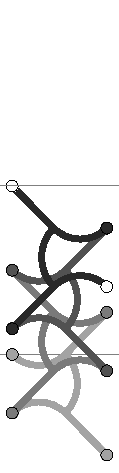
\includegraphics[scale=1]{../Pics/py/straight_f_ori_1.pdf}&
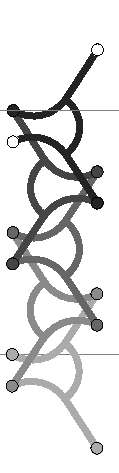
\includegraphics[scale=1]{../Pics/py/straight_f_ori_01.pdf}&
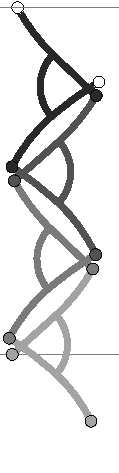
\includegraphics[scale=1]{../Pics/py/straight_f_ori_0001.pdf} \\
(a) & (b) & (c) \\
\end{tabular}
\caption{Optimal straight gait patterns $\bm{R}_\mathcal{S}^2(\bm{y})$ for different parameter sets $\mathcal{P} = [b_\alpha, b_\ell, w_\ell, w_\alpha, w_\varphi]$.
(a) $w_\varphi = 1$, $\bm{y}=[90^\circ~0^\circ~-90^\circ~90^\circ~0^\circ]$.
(b) $w_\varphi = .01$, $\bm{y}=[86^\circ~4^\circ~-110^\circ~83^\circ~4^\circ]$.
(c) $w_\varphi = .0001$, $\bm{y}=[0^\circ~18^\circ~-85^\circ~10^\circ~22^\circ]$.}
\label{fig:opt_straight_gait}
\end{center}
\end{figure}

%Abbildung~\ref{fig:opt_straight_gait} zeigt die Ergebnisse der Optimierung für verschiedene Parametersets $\mathcal{P}$.
%Es sind jeweils die vier Posen aus zwei Zyklen dargestellt.
%Dabei sind die Grenzen der Biegewinkel $b_{\alpha} = 100^\circ$ und Längen $b_{\ell}=.1$ für alle drei Optimierungen konstant.
%Auch die Kosten für Abweichung von Nennlänge $w_\ell = 100$ und Abweichung vom Referenzwinkel $w_\alpha=10$ sind konstant.
%Der einzige Unterschied der drei Simulationen ist der Gewichtungsfaktor der Fußorientierungsabweichung $w_\varphi$.
%In (a) ist $w_\varphi=1$ vergleichweise hoch. 
%Es ist also "teuer" einen fixierten Fuß relativ zur vorhergegangen Pose zu verdrehen.
%Das resultierende optimale Laufmuster, ist das zu $\bm{y}_0$ korrespondierende und schon aus~\cite{PA_Schiller} bekannt.
%Senkt man die Kosten für die Verdrehung der Füße etwas ($w_\varphi=0.01$), so ist das in (b) gezeigte Laufmuster optimal.
%Innerhalb der zwei Zyklen generiet der Roboter im Vergleich zur Simulation in (a) $1.46 \times$ mehr Vorschub.
%Vernachlässigt man die Kosten für die Verdrehung der Füße gänzlich ($w_\varphi=0.0001$), resultiert das in (c) gezeigte Laufmuster.
%Praktisch ist dieser Gang zwar nicht möglich, da der Roboter über seine eigenen Beine stolpern würde, aber als theoretische Spielerei ist durchaus interessant.
%Im Vergleich zu (a) konnte mehr als doppelt soviel ($2.11 \times$) Vorschub erzeugt werden.

Figure~\ref{fig:opt_straight_gait} shows the optimization results for different parameter sets $\mathcal{P} = [b_\alpha, b_\ell, w_\ell, w_\alpha, w_\varphi]$.
The four poses from two cycles are depicted.
The limits of the bending angles $b_{\alpha} = 100^\circ$ and lengths $b_{\ell}=.1$ are constant for all three optimizations.
The costs for deviation from nominal length $w_\ell = 100$ and deviation from reference angle $w_\alpha=10$ are also constant.
The only difference between the three simulations is the weighting factor on the deviation of the feet orientations $w_\varphi$.
In (a) $w_\varphi=1$ is comparatively high. 
It is therefore \textsl{expensive} to twist a fixed foot relative to the previous pose.
The resulting optimal gait pattern is the one corresponding to $\bm{y}_0$ and already known from~\cite{PA_Schiller}.
If the cost of twisting the feet is reduced slightly ($w_\varphi=0.01$), the gait pattern shown in (b) is optimal.
Within the two cycles, the robot generates $1.46 \times$ more shift in position compared to the simulation in (a).
If the cost of twisting the feet is almost neglected ($w_\varphi=0.0001$), the gait pattern shown in (c) results.
Practically this gait is not possible, because the robot would trip over its own legs, but as a theoretical gimmick it is quite interesting.
Compared to (a), more than twice as much ($2.11 \times$) shift in position could be generated.

\subsection{Gait Pattern for a curve}

%Im Gegensatz zum gradlinigen Gang, ist das Laufmuster einer Kurve nicht symmetrisch.
%Die Annahme, dass ein Zyklus aus zwei Posen mit jeweils diagonal gegenüberliegend fixierten Füßen besteht, ist jedoch weiterhin sinnvoll.
%Dementsprechend hat das Laufmuster einer Kurve zehn Unbekannte, nämlich die Referenzwinkel der beiden Posen eines Zyklus.
%Die zu optimierende Variable ergibt sich damit zu:
In contrast to the straight motion, the gait pattern of a curve is not symmetrical.
However, it still reasonable to assume that a cycle consists of two poses, each with diagonally opposite fixed feet.
Accordingly, the running pattern of a curve has ten unknowns, namely the reference angles of the two poses of a cycle.
This results in the variable to be optimized:
\begin{equation}
\bm{z} = 
\begin{bmatrix}
\bm{z}_1 \\ \bm{z}_2
\end{bmatrix}
=
\begin{bmatrix}
\begin{matrix}
\alpha_{\textnormal{ref},1}& \alpha_{\textnormal{ref},2}&\alpha_{\textnormal{ref},3}&\alpha_{\textnormal{ref},4}&\alpha_{\textnormal{ref},5}
\end{matrix}
 \\
\begin{matrix}
\alpha_{\textnormal{ref},6}& \alpha_{\textnormal{ref},7}&\alpha_{\textnormal{ref},8}&\alpha_{\textnormal{ref},9}&\alpha_{\textnormal{ref},10}
\end{matrix}
\end{bmatrix} .
\end{equation}
%Wie zuvor kann nun die Struktur des Laufmuster einer Kurve mit $n$ Zyklen $\bm{R}_\mathcal{C}^n \in \mathbb{R}^{2n\times 9}$definiert werden:
As before, the structure of the gait pattern of a curve with $n$ cycles $\bm{R}_\mathcal{C}^n \in \mathbb{R}^{2n\times 9}$ can now be defined as:
\begin{equation}
\bm{R}_\mathcal{C}^n(\bm{z})
=
\left[
\begin{array}{c}
\bm{r}_1 \\
\bm{r}_2 \\
\hline
\bm{r}_3 \\
\bm{r}_4 \\
\hline
\vdots \\
\hline
\bm{r}_{2n-1} \\
\bm{r}_{2n} \\
\end{array}
\right]
=
\left[
\begin{array}{ccccc cccc}
z_1&z_2&z_3&z_4&z_5&1&0&0&1 \\
z_6&z_7&z_8&z_9&z_{10}&0&1&1&0 \\ 
\hline
z_1&z_2&z_3&z_4&z_5&1&0&0&1 \\
z_6&z_7&z_8&z_9&z_{10}&0&1&1&0 \\ 
\hline
\vdots&\vdots&\vdots&\vdots&\vdots&\vdots&\vdots&\vdots&\vdots \\
\hline
z_1&z_2&z_3&z_4&z_5&1&0&0&1 \\
z_6&z_7&z_8&z_9&z_{10}&0&1&1&0 \\ 
\end{array}
\right] .
\label{eq:gait_ptrn_curve}
\end{equation}

%Um eine Kurve zu laufen ist es optimal die Differenz zwischen der Orientierung der Initialpose $\varepsilon_0$ und jener der Endpose nach $n$ Zyklen $\varepsilon_{2n}$ möglichst zu maximieren bzw. minimieren, je nach dem ob eine Links- oder Rechtskurve gelaufen werden soll.
%Zur Bestimmung der Initialpose $\bm{\rho}_0$ werden die Referenzwinkel der ersten Pose $\bm{z}_1$ des gesuchten Laufmusters $\bm{R}_\mathcal{C}(\bm{z})$ in gleicher Weise verwendet, wie dies schon beim geraden Gang geschah.
%Nun kann die Performance eines Laufmusters für eine Kurve mit $n$ Zyklen mittels folgender Funktion quantifiziert werden:
To run a curve it is optimal to maximize or minimize the difference between the orientation of the initial pose $\varepsilon_0$ and that of the end pose after $n$ cycles $\varepsilon_{2n}$, depending on whether a left or right curve is to be run.
To define the initial pose $\bm{\rho}_0$, the reference angles of the first pose $\bm{z}_1$ of the searched gait pattern $\bm{R}_\mathcal{C}(\bm{z})$ are used in the same way as it already happened for straight gait.
Now the performance of a gait pattern for a curve with $n$ cycles can be quantified using the following objective:
\begin{equation}
\Delta\varepsilon^n(\bm{z})
 = 
\left\lbrace
\begin{array}{l}
\bm{\rho}_0 = 
\left[
\begin{array}{c|c|c}
\bm{z}_1 ~ \bm{\ell}_n ~ \varepsilon_0  & 
\bm{P}(\bm{z}_1, \bm{\ell}_n, \varepsilon_0, \bm{p}_{1,0}) & 
1~0~0~0
\end{array}
\right] \\
\textnormal{for } k = 1, \dots, 2n: \\
\qquad \bm{\rho}_k = \textnormal{fun}_{\mathcal{P}}(\bm{r}_k, \bm{\rho}_{k-1}) \\
\Delta \varepsilon = \varepsilon_{2n} - \varepsilon_0 \\
\end{array}
\right. ,
\end{equation}

%Das Optimale Laufmuster für eine Linkskurve zu einem gegebenen Parameterset $\mathcal{P}$ ist dann die Lösung des Optimierungsproblems:
The optimal gait pattern for a left curve to a given parameter set $\mathcal{P}$ is then the solution to the optimization problem:
\begin{equation}
\min_{\bm{z} \in \mathcal{Z}} ~ -\Delta\varepsilon^n(\bm{z}).
\end{equation}
Here $\mathcal{Z}$ describes the set of allowed values.
All reference angles of the legs should be $z_i\geq0,~i=1,2,4,5,6,7,9,10$. 
The reference angles of the torso $z_i,~i=3,8$ are not constrained, since it can bend into both directions.
%Für eine Rechtskurve multipliziert man die Kostenfunktion mit $-1$.
For a right turn, multiply the objective function by $-1$.
%Zur Lösung des Minimierungsproblems wird wieder ein Startwert benötigt.
%Dafür wird $\bm{z}_0 = [\bm{y}_0~\bm{y}_0]$ gewählt.
A starting value is required again to solve the minimization problem.
Therefore $\bm{z}_0 = [\bm{y}_0~\bm{y}_0]$ is chosen.


%Abbildung~\ref{fig:opt_curve_gait} zeigt die Ergebnisse der Optimierung für verschiedene Parametersets $\mathcal{P}$.
%Es sind jeweils die vier Posen von zwei Zyklen und die erste Pose des dritten Zyklus dargestellt.
%Die Grenzen, sowie die Kosten für Winkel- und Längenabweichung sind in allen Simulationen konstant $[b_\alpha, b_\ell, w_\ell, w_\alpha] = [100^\circ, .1, 100, 10]$.
%Wieder wurden nur die Kosten für die Orientierungsabweichung der fixierten Füße $w_\varphi$ variiert.
%Die ersten drei Abbildungen (a)--(c) zeigen optimale Linkskurven ($\min -\Delta \varepsilon$).
%In ist ein Verdrehen der Füße relativ teuer $w_\varphi=1$.
%Innerhalb der 2.5 Zyklen konnte eine Rotation von $45^\circ$ generiert werden, was $18^\circ/$cycle entspricht.
%Man beachte, dass die Orientierung der fixierten Füße nahezu konstant bleibt.
%In (b) wurden die Kosten für das Verdrehen der Füße etwas gesenkt ($w_\varphi=.1$).
%Die Orientierungsabweichung der fixierten Füße ist nun zwar etwas größer, dafür wurde aber eine Rotation von $30^\circ/$cycle erzeugt, und damit fast Doppelt soviel wie in (a).
%In (c) besitzt der Roboter quasi voll bewegliche Fußgelenke ($w_\varphi=.0001$).
%In den den 2.5 Zyklen rotiert er um $235^\circ \hat{=} 94^\circ/$cycle.
%Allerdings beinhaltet dieses Laufmuster Biegewinkel von bis zu $221^\circ$, sodass es praktisch schwer umzusetzen ist.

Figure~\ref{fig:opt_curve_gait} shows the optimization results for different parameter sets $\mathcal{P}$.
The four poses of two cycles and the first pose of the third cycle are shown.
The limits and costs for angle and length deviation are constant $[b_\alpha, b_\ell, w_\ell, w_alpha] =[100^\circ, .1, 100, 10]$ in all simulations.
Again, only the cost of the orientation deviation of the fixed feet $w_\varphi$ was varied.
The first three figures (a)--(c) show optimal left curves ($\min -\Delta \varepsilon$).
In (a), twisting of the feet is relatively expensive $w_\varphi=1$.
Within the 2.5 cycles a rotation of $45^\circ$ could be generated, which corresponds to $18^\circ/$cycle.
Note that the orientation of the fixed feet remains almost constant.
In (b) the cost of twisting the feet was slightly reduced ($w_\varphi=.1$).
The orientation deviation of the fixed feet is now slightly larger, but a rotation of $30^\circ/$cycle was generated, almost twice as much as in (a).
In (c) the robot has almost fully movable ankle joints ($w_\varphi=.0001$).
In the 2.5 cycles it rotates around $235^\circ \hat{=} 94^\circ/$cycle.
However, this gait pattern has a bending angles of up to $221^\circ$, making it practically difficult to move.

%Die Abbildungen (d)--(f) zeigen optimale Rechtkurven ($\min \Delta \varepsilon$) für verschieden steife Fixierungsaktuatoren.
%Genau wie für die Linkskurven steigt die Rotation/Zyklus mit sinkender Steifigkeit $w_\varphi$.
%Interessant hierbei ist jedoch, dass der Roboter nun rückwärts läuft.
%Dies lässt sich durch den Anfangswert $\bm{z}_0 = [\bm{y}_0~\bm{y}_0]$ des Optimierungsproblem erklären.
%Da die initialen Referenzwinkel des Torso $z_3, z_8 < 0$ sind, ist der Torso initial nach links gekrümmt. 
%Diese Krümmung, beziehungsweise das Vorzeichen, bleibt während der ganzen Optimierung erhalten.
%Soll der Roboter nach vorne rechts laufen, so müssen die Referenzwinkel gespiegelt werden.
%Das Spiegelbild $\tilde{\bm{r}}$ eines Referenzinputs $\bm{r}$ ist definiert als:
The figures (d)--(f) show optimal right curves ($\min \Delta \varepsilon$) for differently stiff fixation actuators.
As for the left curves, the rotation/cycle increases with decreasing stiffness $w_\varphi$.
What is interesting here, however, is that the robot now runs backwards.
This can be explained by the initial value $\bm{z}_0 = [\bm{y}_0~\bm{y}_0]$ of the optimization problem.
Since the initial reference angles of the torso are $z_3, z_8 < 0$, the torso is initially curved to the left. 
This curvature, or the sign, is retained throughout the entire optimization.
If the robot is to run forward right, the reference angles must be mirrored.
The mirror image $\tilde{\bm{r}{r}}$ of a reference input $\bm{r}$ is defined as:
\begin{equation}
\tilde{\bm{r}}(\bm{r}) = \begin{bmatrix}
r_2 & r_1 & - r_3 & r_5 & r_4  & \bm{f}
\end{bmatrix} .
\end{equation}
%Wendet man die Spiegelung auf alle Posen der Laufmuster für Rechtskurven an, läuft der Roboter nach vorne rechts.
If the mirroring is applied to all poses of the gait pattern for right turns, the robot runs forward right.

\begin{figure}
\begin{center}
\begin{tabular}{ccc}
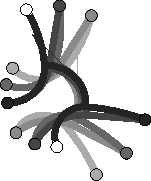
\includegraphics[scale=1]{../Pics/py/Curve_f_ori_1.pdf}&
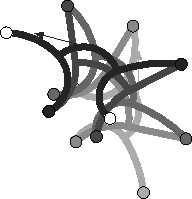
\includegraphics[scale=1]{../Pics/py/Curve_f_ori_01.pdf}&
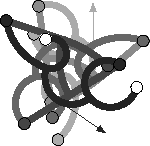
\includegraphics[scale=1]{../Pics/py/Curve_f_ori_0001.pdf}\\
(a) & (b) & (c)\\
\end{tabular}

\begin{tabular}{ccc}
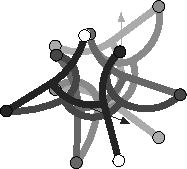
\includegraphics[scale=1]{../Pics/py/U-turn_f_ori_1.pdf}&
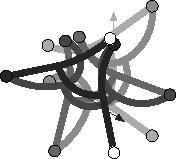
\includegraphics[scale=1]{../Pics/py/U-turn_f_ori_01.pdf}&
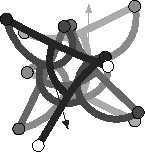
\includegraphics[scale=1]{../Pics/py/U-turn_f_ori_0001.pdf} \\
(d) & (e) & (f)\\
\end{tabular}
\caption{
Optimal left curve gait patterns $\bm{R}_\mathcal{C}^2(\bm{z})$ for different parameter sets $\mathcal{P} = [b_\alpha, b_\ell, w_\ell, w_\alpha, w_\varphi]$ ($\min -\Delta\varepsilon$):
(a) $w_\varphi = 1$, $\bm{z}=[[97^\circ~28^\circ~-98^\circ~116^\circ~17^\circ]~[79^\circ~0^\circ~-84^\circ~67^\circ~0^\circ]$.
(b) $w_\varphi = .1$, $\bm{z}=[[104^\circ~48^\circ~-114^\circ~124^\circ~27^\circ]~[72^\circ~0^\circ~-70^\circ~55^\circ~0^\circ]$.
(c) $w_\varphi = .0001$, $\bm{z}=[[164^\circ~124^\circ~-152^\circ~221^\circ~62^\circ]~[0^\circ~0^\circ~-24^\circ~0^\circ~0^\circ]$.
Optimal right curve gait patterns ($\min \Delta\varepsilon$):
(d) $w_\varphi = 1$, $\bm{z}=[[63^\circ~0^\circ~-72^\circ~46^\circ~0^\circ]~[114^\circ~77^\circ~-121^\circ~144^\circ~31^\circ]$.
(e) $w_\varphi = .01$, $\bm{z}=[[60^\circ~0^\circ~-70^\circ~30^\circ~0^\circ]~[110^\circ~70^\circ~-132^\circ~149^\circ~43^\circ]$.
(f) $w_\varphi = .001$,  $\bm{z}=[[50^\circ~0^\circ~-51^\circ~6^\circ~0^\circ]~[121^\circ~92^\circ~-146^\circ~167^\circ~54^\circ]$.
}
\label{fig:opt_curve_gait}
\end{center}
\end{figure}




\section{Case Study}

Apply the gait patterns on the real robot an evaluate the performance.



\clearpage
\appendix
\section{Appendix}

\begin{multicols}{2}

\begin{equation}
r_i = \frac{360 ~ \ell_i}{2 \pi ~ \alpha_i},~~ \textnormal{for}~ i \in [1,2,3,4,5]
\label{eq:F1_start}
\end{equation}

\begin{equation}
\bm{\varphi} = \begin{bmatrix}
\varepsilon - \alpha_1 - \frac{1}{2}\alpha_3 \\
\varphi_1 + \alpha_1 + \alpha_2 \\
180^\circ + \alpha_3 - \alpha_2 + \alpha_4 + \varphi_2 \\
180^\circ + \alpha_3 - \alpha_1 + \alpha_5 + \varphi_1 \\
\end{bmatrix}
\label{eq:phi_calc}
\end{equation}

If $f_1$:

\begin{equation}
\bm{p}_{R1} = \bm{p}_1 + 
\begin{bmatrix} 
\cos(\varphi_1)\\ 
\sin(\varphi_1)\end{bmatrix} r_1
\end{equation}

\begin{equation}
\bm{p}_{OM} = \bm{p}_{R1} + \begin{bmatrix} 
\cos(\varphi_1 + \alpha_1) \\ 
\sin(\varphi_1 + \alpha_1)
\end{bmatrix} r_1
\end{equation}

\begin{equation}
\bm{p}_{R2} = \bm{p}_{OM} + 
\begin{bmatrix} 
\cos(\varphi_1 + \alpha_1) \\ 
\sin(\varphi_1 + \alpha_1)
\end{bmatrix} r_2
\end{equation}

\begin{equation}
\bm{p}_{2} = \bm{p}_{R2} + 
\begin{bmatrix} 
-\cos(\varphi_2) \\ 
-\sin(\varphi_2)
\end{bmatrix} r_2
\end{equation}



If $f_2$:

\begin{equation}
\bm{p}_{R2} = \bm{p}_{2} + 
\begin{bmatrix} 
\cos(\varphi_2) \\ 
\sin(\varphi_2)
\end{bmatrix} r_2
\end{equation}

\begin{equation}
\bm{p}_{OM} = \bm{p}_{R2} + 
\begin{bmatrix} 
-\cos(\varphi_2-\alpha_2) \\ 
-\sin(\varphi_2-\alpha_2)
\end{bmatrix} r_2
\end{equation}

\begin{equation}
\bm{p}_{R1} = \bm{p}_{OM} + 
\begin{bmatrix} 
\cos(\varphi_2-\alpha_2) \\ 
\sin(\varphi_2-\alpha_2)
\end{bmatrix} r_1
\end{equation}

\begin{equation}
\bm{p}_{1} = \bm{p}_{R1} + 
\begin{bmatrix} 
-\cos(\varphi_1) \\ 
-\sin(\varphi_1)
\end{bmatrix} r_1
\end{equation}


Both:

\begin{equation}
\bm{p}_{RM} = \bm{p}_{OM} + \begin{bmatrix} 
\sin(\varphi_1 + \alpha_1) \\ 
-\cos(\varphi_1 + \alpha_1) \end{bmatrix} r_3
\end{equation}


\begin{equation}
\bm{p}_{UM} = \bm{p}_{RM} + \begin{bmatrix} 
- \cos(\alpha_3 - 90 + \varphi_1 + \alpha_1) \\ 
- \sin(\alpha_3 - 90 + \varphi_1 + \alpha_1) \end{bmatrix} r_3
\end{equation}

\begin{equation}
\bm{p}_{R4} = \bm{p}_{UM} + \begin{bmatrix} 
\sin(\alpha_3 - 90 + \varphi_1 + \alpha_1) \\
- \cos(\alpha_3 - 90 + \varphi_1 + \alpha_1) \end{bmatrix} r_4
\end{equation}

\begin{equation}
\bm{p}_{4} = \bm{p}_{R4} + \begin{bmatrix} 
-\cos(\varphi_4) \\
-\sin(\varphi_4)\end{bmatrix} r_4
\end{equation}

\begin{equation}
\bm{p}_{R3} = \bm{p}_{UM} + \begin{bmatrix} 
\sin(\alpha_3 - 90 + \varphi_1 + \alpha_1) \\
 - \cos(\alpha_3 - 90 + \varphi_1 + \alpha_1) \end{bmatrix} r_3
\end{equation}

\begin{equation}
\bm{p}_{3} = \bm{p}_{R3} + \begin{bmatrix} 
- \cos(\varphi_3)\\
- \sin(\varphi_3)\end{bmatrix}r_3
\label{eq:F1_end}
\end{equation}

\end{multicols}


\begin{figure}[h]
\begin{center}

\begin{tabular}{ccc}
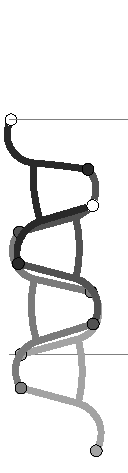
\includegraphics[scale=1]{../Pics/py/n_belly_100_10_001.pdf}&
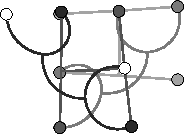
\includegraphics[scale=1]{../Pics/py/U-turn.pdf}&
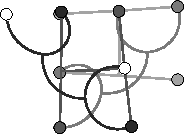
\includegraphics[scale=1]{../Pics/py/U-turn.pdf} \\
(a) & (b) & (c)\\
\end{tabular}

\caption{
(a) Optimal straight gait patterns without moving torso $\mathcal{P} = [100, .1, 100, 10, .001]$.
(b) Optimal curve for a fixed initialpose with $\bm{\alpha}_0 = [0~0~0~0~0]$, $w_\varphi = .0001$, $\bm{z}=[[0^\circ~0^\circ~-7^\circ~0^\circ~0^\circ]~[114^\circ~109^\circ~-101^\circ~146^\circ~82^\circ]$.
(c) Space for more 
}
\label{fig:straight_gait_no_torso}
\end{center}
\end{figure}



\end{document}